\documentclass[11pt,letterpaper]{article}
\usepackage{amsmath,amssymb}
\usepackage{framed}
\usepackage{mdframed}
% Use adjustwidth environment to exceed column width (see example table in text)
\usepackage{changepage}
\usepackage[font={small}]{caption}

\DeclareUnicodeCharacter{0301}{*************************************}
% textcomp package and marvosym package for additional characters
\usepackage{textcomp,marvosym}
\usepackage[T1]{fontenc}
\usepackage{lmodern}
\usepackage{todonotes}
% cite package, to clean up citations in the main text. Do not remove.
%\usepackage{cite}
% Use nameref to cite supporting information files (see Supporting Information section for more info)
\usepackage{svg}
\usepackage{svg-extract}
\usepackage[hidelinks]{hyperref}
\usepackage{nameref}%
\usepackage{float}
\usepackage[section]{placeins}
\usepackage[backend=biber,style=vancouver]{biblatex}
\addbibresource{export.bib} %Import the bibliography file
%\usepackage[right]{lineno}
\usepackage{adjustbox}
\usepackage[nopatch=eqnum]{microtype}
\DisableLigatures[f]{encoding = *, family = * }
% array package and thick rules for tables
\usepackage{array}

% create "+" rule type for thick vertical lines
\newcolumntype{+}{!{\vrule width 2pt}}

% create \thickcline for thick horizontal lines of variable length
\newlength\savedwidth
\newcommand\thickcline[1]{%
  \noalign{\global\savedwidth\arrayrulewidth\global\arrayrulewidth 2pt}%
  \cline{#1}%
  \noalign{\vskip\arrayrulewidth}%
  \noalign{\global\arrayrulewidth\savedwidth}%
}

% \thickhline command for thick horizontal lines that span the table
\newcommand\thickhline{\noalign{\global\savedwidth\arrayrulewidth\global\arrayrulewidth 2pt}%
\hline
\noalign{\global\arrayrulewidth\savedwidth}}

% Remove comment for double spacing
\usepackage{setspace} 
\doublespacing

% Text layout
%%\raggedright
%%\setlength{\parindent}{0.5cm}
%\textwidth 5.25in 
%\textheight 8.75in

% Bold the 'Figure #' in the caption and separate it from the title/caption with a period
% Captions will be left justified
\usepackage[aboveskip=1pt,labelfont=bf,labelsep=period,justification=raggedright,singlelinecheck=off]{caption}
\renewcommand{\figurename}{Fig}

% Use the PLoS provided BiBTeX style
%\bibliographystyle{plos2015}

% Remove brackets from numbering in List of References
\makeatletter
\renewcommand{\@biblabel}[1]{\quad#1.}
\makeatother

% Header and Footer with logo
\usepackage{lastpage,fancyhdr,graphicx}
\usepackage{epstopdf}
%\pagestyle{myheadings}
\pagestyle{fancy}
\fancyhf{}
%\setlength{\headheight}{27.023pt}
%\lhead{\includegraphics[width=2.0in]{PLOS-submission.eps}}
\rfoot{\thepage/\pageref{LastPage}}
\renewcommand{\headrulewidth}{0pt}
\fancyhf{}
\fancyhead[C]{\thepage}
\renewcommand{\headrulewidth}{0pt}
\pagestyle{fancy}
%\renewcommand{\footrule}{\hrule height 2pt \vspace{2mm}}
%\fancyheadoffset[L]{2.25in}


%% END MACROS SECTION

\usepackage[left=2.5cm,top=3cm,right=2.5cm,bottom=3cm,bindingoffset=0.5cm]{geometry}
\begin{document}
\vspace*{0.2in}

% Title must be 250 characters or less.
\begin{flushleft}
{\Large
\textbf\newline{Radial control of cryptic pathogens invading  multi-type populations} % Please use "sentence case" for title and headings (capitalize only the first word in a title (or heading), the first word in a subtitle (or subheading), and any proper nouns).
}
\newline
% Insert author names, affiliations and corresponding author email (do not include titles, positions, or degrees).

Alexis Vargas Richards 
\bigskip
\newline Girton College, ar2185
\newline
Supervisor: Prof NJ Cunniffe 
\newline word count: 5997 words 
\bigskip


\end{flushleft}

\newpage
% Please keep the abstract below 300 words
\section*{Abstract}

Invasive plant diseases cause crop damage across the world. Plant pathogens may infect, transmit or show symptoms differently across host species. I formulate a stochastic multi-type small-scale model for an invading disease subject to periodic survey-based detection, and removal of hosts within a control radius. The parameterisation is to the bacterial phytopathogen \emph{Xylella fastidiosa}, which infects multiple host species including olives, and causes major economic damage. I find that different forms of crypticity (either longer cryptic infection or lower symptom detection probability) reduce control efficacy, and this is particularly pronounced when the alternate, cryptic host is present at high frequency.


\bigskip
%We find that for unclustered and clustered landscapes, a small proportion of %cryptic% h%osts leads to a nonlinear breakdown in single-radius control in a subset of %parameterisations. This is modulated in significant ways by the patterning of the hosts as well as asymmetric transmission.
% Please keep the Author Summary between 150 and 200 words


\textbf{Key words}: Optimal control, plant disease, Xylella, host heterogeneity, parameter misspecification

\section*{Author summary}

Invading plant diseases can cause significant damage to crop systems,  ecosystems and economies alike. To mitigate this, costly disease control programmes are often deployed. However, these meet with varying levels of success. The design of control schemes such as removing potential hosts within a fixed distance of a detected infection depends upon knowing which hosts can transmit the infection and when they show symptoms if infected (if they show symptoms at all). If a second host type can also be infected and transmit the disease, perhaps taking a longer time to show symptoms or showing difficult-to-spot symptoms, then I show using a modelling approach that the control programme can perform badly. Throughout this work I draw a contrast between the local impacts of an epidemic due to removing hosts, and the potential for a given outbreak to infect areas adjacent to those I consider directly (particularly undesirable for disease making a first incursion into an area). The results have significance for the control of invasive plant diseases across the world, particularly for the economically damaging bacterial disease olive quick decline syndrome (OQDS), to which the model is parameterised. They suggest that a successful control programme should be designed with the potential for transmission across host types in mind, and that the multiple ways for infection to go undetected can hamper disease control based on removing hosts within a certain distance of a detected infection.

\section*{Introduction}

Epidemics of plant disease have occurred throughout history, to the detriment of economies, ecosystems and food security alike \cite{Boyd2013}. Controlling the establishment of invasive pathogens is an  especially pressing issue given that frequency of the resulting epidemics has increased over the last 100 years \cite{Montgomery2023} and threatens food production \cite{Fones2020, Ristaino2021}. However, how best to control invading plant disease is not a trivial question. The challenge is not only to identify an optimal strategy but also to reconcile this with real-world communicability \cite{Cunniffe2015}, and economic limits on which control regimes are feasible and which are financially or technically prohibitive, especially in resource-poor settings \cite{Jeger2021}. Furthermore, the control problem becomes less tractable when cryptically infected hosts are present \cite{Filipe2012}: these hosts may infect others while not displaying symptoms \cite{Lee2015}, or display symptoms which have a small probability of detection. Uncertainty in epidemiological parameters \cite{Cunniffe2015, Habibzadeh2010}, in the observation of system states \cite{McClintock2010} or in models more generally \cite{Christley2013} also poses challenges for control regimes.

Modelling multi-host pathogens has also been highlighted as a key challenge in disease ecology \cite{Buhnerkempe2015}, and multiple important plant pathogens infect more than one species, including etiologic agents of Asiatic citrus canker \cite{Pruvost2022} and sudden oak death (SOD) \cite{Grunwald2008} and the Tomato spotted wilt virus (TWSV) \cite{Parrella2003}. Notably, different host species or cultivars (henceforth 'types') may exhibit different rates of symptom emergence (if they display symptoms) and may transmit with different propensities \cite{Bragard2019, NdeffoMbah2010}. Differential pathogen detectability across hosts complicates finding an optimal control strategy, and there may be questions over the extent to which alternate hosts contribute to transmission in ongoing epidemics: for instance in Cacao swollen shoot virus (CSSV) in Ghana it is unknown to what extent wild plants transmit the virus \cite{Ameyaw2024}.

The pathogen motivating this modelling study, \emph{Xylella fastidiosa}, is an emerging multi-host bacterium currently causing severe economic losses in Europe \cite{Bodino2021,Martelli2016}. It is projected to cause future economic damage (up to billions of euros) to olive production over the next 50 years, through extensive olive tree infection by variety CoDiRo (sequence type 53 of subsp. \emph{pauca}) which causes Olive Quick Decline Syndrome (OQDS) \cite{Marcelletti2016,Schneider2020}. Infected olive trees become desiccated and die, reducing yield. Further economic modelling suggests that spread of \emph{X. fastidiosa}  will have negative effects on EU consumers (as well as farmers) due to higher prices of olive products \cite{Schneider2021}. Aside from OQDS, \emph{X. fastidiosa} is also responsible for several other diseases of major agricultural importance, such as Pierce's disease of grapevine \cite{GimenezRomero2024} and almond leaf scorch (ALS) \cite{Gibin2023}. the susbpecies \emph{pauca} is currently known to infect at least several hundred species of plants \cite{Gibin2023}, and is a pathogen of major concern across the European Union due to its proven capability to damage a variety of species. In Mallorca, for instance, approximately 81\% of almond trees are infected by almond leaf scorch (caused by \emph{X. fastidiosa} subsp. \emph{fastidiosa} and subsp. \emph{multiplex}), perhaps following import of infected scions from California \cite{Olmo2021}. The ensuing dramatic landscape impacts (scorching, desiccation and death of trees) are obviously undesirable \cite{GimenezRomero2023}. 

A profusion of \emph{X. fastidiosa} models have been published. For instance, a large spatial scale model (400 km by 80 km) was formulated in \cite{Anita2021} to assess efficacy of control applied to a spatial subdomain of the landscape. The model does describe the effect of weed-like vegetation on the abundance of vectors, but no account was made for potential transmission between this alternate vegetation and the crop which is infected. There was also no consideration of host crypticity and the model did not deal in individual hosts but rather densities of hosts. A similarly large-scale model \cite{Cendoya2024} used a gridded approach to examine the effect of control interventions on almond scorch disease in Alicante, Spain. However, that model approximated transmission using a grid, and here a more exact (fully individual-based) approach is used coupled with addition of a second host type. 

Current EU legislation mandates the removal of all susceptible hosts within a 100m radius of a detected \emph{X.fastidiosa} infection \cite{Bragard2019}. Removal of potential hosts within a given radius of detected infection has historical precedent, for instance in a control programme against \emph{Phytophthora ramorum} in Oregon, where host removal took place within a radius of 100-200 metres \cite{Hansen2019}. A radial control scheme was also used in the control of Asiatic citrus canker (ACC) in Brazil, with an initial removal radius of 12m used from 1957 and subsequently increased to 1000m in 1962 \cite{Behlau2016}. Similarly in Florida, control of invasive citrus canker initially used a radius of 38 m (the '125ft rule') after preliminary studies suggested pathogen dispersal distance of only up to 32 m, but this was increased to 579 m ('1900ft rule') in late 1999, following more thorough dispersal studies and consideration of extreme weather events \cite{Gottwald2001}. Control was finally abandoned several years later. The failure of the Floridian citrus canker control programme illustrates the importance of accurate knowledge in formulating successful controls for invasive plant disease, or indeed attempting disease control at all. The present work explores further what happens to control when the unknown aspect of the system is the fraction of type B hosts which are defined as being more cryptic (less visible to control while infectious) than type A hosts. 

 Misspecification of epidemiological parameters due to incomplete information is an important scenario in disease control \cite{Cunniffe2015, HyattTwynam2017}, and therefore this work also aims to explore the differential degradation in efficacy of strategies to control invasive infectious disease under partially characterised parameters for different landscapes. Here, observation of host type heterogeneity (i.e., fraction of a second host type) and imperfect control regimes are used to explore the potential for differences in disease control efficacy in field settings. To this end, the system simulated is at a smaller scale than other studies, for computational tractability and to examine the effect of different management strategies on a olive grove-like scale. 
\begin{framed}
	\subsection*{ \label{question} Key Questions}
\begin{itemize}
	
   \item[\textbf{Q1}] \label{Q1} How does varying the proportion of host type A (less cryptic) and host type B (more cryptic) affect control? 
   
   \item[\textbf{Q2}] \label{Q2} What is the divergence between an approach optimised to each landscape case, versus a control strategy optimised to a single host type landscape? 
   
%     \item[\textbf{Q3}] \label{Q3} {Does the nature of increased crypticity (i.e., either lower detection probability or longer cryptic period) make a difference to disease controllability? }
  %  \item[\textbf{Q3}] \label{Q3} Are there nonlinearities in the breakdown of control as landscape or host parameters change? Are these present in both the parameter misspecification case and the landscape-optimised case?
   % \item[\textbf{Q3}] \label{Q4} {How do different host landscapes modulate the above effects, with respect to the density of hosts and their clustering?}
    \item[\textbf{Q3}] \label{Q3} {How does asymmetric transmission affect the efficacy of control?}
    
\end{itemize}
\end{framed}

\FloatBarrier
\section*{Methods}

\subsection*{Generating Host Landscapes}

\textbf{CSR}: Complete Spatial Randomness
\newline
\label{csr}
    Hosts are distributed according to random numbers generated with uniform probability on the [0,1] interval for the x- and y-coordinates, and multiplied by $L$ (metres) to give a position (x , y) metres on a square of side length $L$ m and area $L^2$ m$^2$. The probability distribution for the position of each point is independent. The fraction of each host type is varied as desired giving a metric, frac(B) = number of B hosts divided by the total number of hosts (type A or B) on the landscape.
   \textbf{Fig. \ref{landscapeexample}} shows two example landscapes with different fractions of type-B hosts. Panel \textbf{(A)} is a type-heterogeneous landscape whereas panel \textbf{(B)} only has type A hosts. 
   
\begin{figure} 
	\centering
    \includesvg[width=\textwidth]{examples}
    \caption{   \label{landscapeexample} \textbf{Examples of landscape instances with different fraction of host type B, frac(B).} \newline \textbf{(A)}: Landscape of complete spatial randomness (CSR) with frac(B) = 0.5, i.e.,  equal numbers of A (blue circle) and B (orange square) hosts. \textbf{(B)}:  CSR landscape with frac(B) = 0 (all hosts are of type A). All landscapes shown here have $N = 1110$, area 16 km$^2$ and thus host density = 69.3 hosts /km$^{2}$.}
\end{figure}

\FloatBarrier
\subsection*{Epidemic Model}

The model is an individual-based,  spatial, stochastic, and has Susceptible-Cryptic-Infected-Removed (SCIR) compartments following \cite{HyattTwynam2017} for the single host-type case.

Hosts may move between the following compartments: $S$, $C$, $I$ and $R$.

\begin{equation}
	S(t) + C(t) + I(t) + R(t) = N(t) = N,   \forall t \ge 0 
\end{equation}

At time $t = 0$, $C_0$ hosts are randomly infected. The $C_{0}$ hosts are cryptic: they do not show symptoms but may transmit infection to other hosts. A preexisting control programme involves surveys of the host population at a frequency every $\Delta$ days, and a symptomatically infected host of type $i$ is detected with probability $p_{d,i}$. The time of the first control event, $\Delta_{0}$ days, is randomly selected from the interval $[0, \Delta]$ days, to reflect an ongoing programme aimed at preventing the establishment of invasive plant disease, and to recapitulate the unpredictability of when an incursion of pathogenic material may occur. If the host is cryptically infected the infection is detected with probability 0, and with $p_{d, i}$ for host of type $i$ in compartment I (symptomatic infected hosts). The number of each host type detected during a round of control is drawn from a binomial distribution with probability of success $p_{d,i}$.

If it is detected, the symptomatic host is removed, along with any other host within a radius of $r$ m. The single host type model corresponds exactly to the case of constant-radius control examined in \cite{HyattTwynam2017}, where $r$ is optimised with respect to an outcome variable. However, to model the propensity for \emph{Xylella fastidiosa} to infect multiple host species or cultivars, the single-host type model was extended to multi-type model with two host types, denoted as A (less cryptic) and B (more cryptic) respectively. The transmission of infectious propagules from species A $\rightarrow$ B may occur with a different propensity than B $\rightarrow$ A, or A $\rightarrow $A (asymmetric transmission). One way to parameterise the asymmetric transmission is as in \cite{NdeffoMbah2010}, where the transmission matrix is 

\begin{equation}
\label{ndeffo}
\begin{pmatrix}
\beta_{AA} & \beta_{AB} \\
\beta_{BA} & \beta_{BB}
\end{pmatrix} 
\end{equation}

with $\beta_{ij}$ the transmission parameter from species $i \rightarrow j$. For the below model, we adopt a more biologically inspired parameterisation, not mathematically distinct from Eq. (\ref{ndeffo}). The constant parameterising transmission from individuals of species $i$ to $j$, $\beta_{ij}$, is a product of both the infectivity of the $i$ species, $\nu_{i}$, and  the susceptibility to infection of the $j$ species, $\phi_{j}$.

\begin{equation}
\beta_{ij} = \nu_{i} \phi_{j}
\end{equation}

and for $j \rightarrow i$:

\begin{equation}
\beta_{ji}= \nu_{j} \phi_{i}
\end{equation}

Therefore:

\begin{equation}
    \begin{pmatrix}
\beta_{AA} & \beta_{AB} \\
\beta_{BA} & \beta_{BB}
 
\end{pmatrix} = 
\begin{pmatrix}
\nu_{A} \phi_{A} & \nu_{A} \phi_{B} \\
\nu_{B} \phi_{A} & \nu_{B} \phi_{B} \\
\end{pmatrix}
\end{equation}

We also incorporate type-specific crypticity, since different host type may to manifest symptoms at different times after infection (reflected by differing $\sigma_{i}$) and potentially to different extents ( differing probability of detection, $p_{d,i}$). Cryptically infected hosts of type $i$ develop symptoms at rate $\sigma_i$ days$^{-1}$. All symptomatic infecteds die at a rate $\gamma$ days$^{-1}$ and move to the Removed ('Dead') compartment.

The stochastic dynamics in the absence of control are thus governed by equations (\ref{twospecies}-\ref{lastone}), where $\Psi_{i}(X \rightarrow Y)$ denotes the transition rate of an individual $i$ from compartment $X$ to compartment $Y$:

%\end{eqnarray}array}

    
%\end{equation}
\begin{eqnarray}    
	\label{twospecies}
\Psi_{i} \left( S_{A} \rightarrow C_{A}\right) &=& \phi_{A} \left( \nu_{A} \left( \sum_{j \in \{C_{A}(t), I_{A}(t)\}}^{}  K(d_{ij}; \alpha) \right) + \nu_{B} \left(\sum_{j \in \{C_{B}(t), I _{B}(t) \}}^{} K(d_{ij}; \alpha) \right) \right) \\
   \Psi_{i} \left( C_{A} \rightarrow I_{A}\right)  &=&  \sigma_{A} \\
   \Psi_{i} \left(I_{A} \rightarrow R _{A}\right) &=& \gamma \\
%\label{twospeciesB}
    \Psi_{i} \left( S_{B} \rightarrow C_{B}\right) &=& \phi_{B} \left( \nu_{A} \left( \sum_{j \in \{ C_{A}(t), I_{A}(t) \}}^{} K(d_{ij}; \alpha) \right) + \nu_{B} \left(\sum_{j \in \{C_{B}(t), I _{B}(t) \}}^{} K(d_{ij}; \alpha) \right) \right) \\
   \Psi_{i} \left( C_{B} \rightarrow I_{B}\right) &=&  \sigma_{B} \\
  \Psi_{i} \left(I_{B} \rightarrow R_{B}\right) &=& \gamma  \label{lastone}
\end{eqnarray}

and the summation index $j \in \{C_{A}(t), I_{A}(t) \}$ is over all hosts $j$ in the set of Cryptics ($C_A$) and Symptomatic Infecteds ($I_{A}$) of type A at time $t$, for instance.
The rate equations Eqs. (\ref{twospecies} - \ref{lastone}) correspond to the flow diagram \textbf{Fig. \ref{compartmentdiag}}.

\begin{figure}
	\centering
	\includesvg[width=\textwidth]{compartment}
	\vspace*{5mm}
	\caption{ \label{compartmentdiag} \textbf{Compartmental diagram of the multitype SCIR model in the absence of control events.} $S_i$ (green fill): Susceptible hosts of type $i$. Both $C_i$ (cryptically infected hosts, yellow fill) may transmit infection to susceptibles of either type with infectivity $\nu_{i}$. Susceptibles of type $i$ are vulnerable to infection with susceptibility $\phi_{i}$. The progression rate of $C_{i}$ to $I_{i}$ (symptomatic infecteds, red fill) is governed by the type-specific rate parameter $\sigma_{i}$. Following symptom development, hosts die at a rate $\gamma$ equal for both types. Dead hosts are in the removed compartment ($R_{i}$, grey fill) and are permanently inactive.}
	\end{figure}

The kernel functions $K(d_{ij}; \alpha)$ considered are the thick-tailed Cauchy kernel and the thin-tailed exponential kernel, which have the forms given in \cite{HyattTwynam2017}. Both functions are parameterised by the dispersal scale $\alpha$, although the Cauchy kernel gives a higher probability of long-distance dispersal events than the exponential kernel.
The system is simulated stochastically using Gillespie's Direct Simulation Algorithm \cite{Gillespie1977} as outlined in \cite{Keeling2008}.

\FloatBarrier
\subsection*{Model parameterisation from \emph{Xylella} studies}

The model formulated here is not predictive. However, efforts have been made to place parameter values within biotic ranges so that the qualitative dynamics of the control problem can be examined. 

\subsubsection*{Crypticity Parameters: Cryptic period parameter $\sigma$ and Probability of Symptom Detection $p_{d}$}
  The European Food Safety Authority (EFSA) provides several species-specific estimates for $\sigma_{i}$ in \cite{Bragard2019}. Specifically, the estimated mean asymptomatic time is $\frac{1}{452}$ days$^{-1}$ for \emph{Olea europea} infected by \emph{X. fastidiosa} subsp. \emph{pauca}. However, the estimated median asymptomatic time for this pathosystem via parametric and non-parametric methods respectively given in \cite{Bragard2019} lead to estimates of $\frac{1}{203}$ and $\frac{1}{452}$ days$^{-1}$ for the asymptomatic period. The difference between these suggests that the parameter estimates are not very precise. An additional complexity is that the SCIR model assumes that hosts are instantaneously infectious to others following infection, but this is not realistic \cite{Leclerc2014}. Instead, there is a non-zero incubation time, not explicitly modelled here. In view of the considerable uncertainty on precise quantification and in addition the simplistic nature of exponentially distributed residence time in the Cryptic compartment, $\sigma$ is set to $\frac{1}{350}$  days$^{-1}$ for host type A, which represents an olive-like host. This is between the values derived via the two different estimation methods from EFSA.
  An alternative value for host type B  $\frac{1}{500} \mathrm{days^{-1}}$ (more cryptic)  was arbitrarily chosen, but is well within the range of vales for different pathosystems in \cite{Bragard2019}.
  
  The probability of symptom detection in type B hosts $p_{d, B}$ was set to 1 or 0.2. These were arbitrary choices, reflecting the potential for lack of recognition of symptoms on alternative hosts. $p_{d,A}$ was set as 1 in light of the obviousness of OQDS-related desiccation on \emph{O. europaea}. 
  
\FloatBarrier
\subsubsection*{Dispersal Kernel and Scale Parameter of \emph{Xylella fastidiosa}}

In \cite{White2017}, a grid-based approach was used to model the early spread of \emph{X. fastidiosa} in Apulia, Italy. Two dispersal kernels of different scales were combined in that work. A simpler approach taken here is the use of a single kernel, either the thicker-tailed Cauchy dispersal kernel, or the thinner-tailed exponential kernel which is $K_{\exp}(d; \alpha) = \exp\left(\frac{-d}{\alpha}\right)$ as in \cite{HyattTwynam2017}. 

\emph{Xylella fastidiosa} is primarily vectored in the European Union (EU) by the spittlebug \emph{Philaenus spumarius} \cite{Bragard2019, Bodino2021}. A Mark-Release-Recapture technique was used in \cite{Bodino2021} to estimate a Gaussian dispersal kernel at different times following vector release. 50\% of spittlebugs stayed within 200m over the course of 6 months in an olive grove setting in Apulia, Italy. Using the cumulative distribution function formula (CDF) for a 2D normalised exponential dispersal kernel, this median value implied a scale parameter of 119 m for the exponential kernel. Since the Cauchy kernel $K(d_{ij}; \alpha) = \frac{1}{1+\left(\frac{d_{ij}} {\alpha}\right)^2}$ cannot be normalised in $\mathbb{R}^2$, the scale parameter for this kernel was derived via least-squares fitting to the exponential kernel ($\alpha_{\mathrm{expon.}}=119$m), giving a scale parameter for the Cauchy kernel of $\alpha_{\mathrm{cauchy}}= 84.5$m.
In the short range eco-epidemiological model \cite{Bragard2019}, susceptibility of the host plant was defined by as the average probability a host is systemically infected following 1 day of feeding by an infected vector. Hence, asymmetric transmission was implemented as type A having lower susceptibility than type B. In symmetric cases, the value of $\phi_{i}$ was set equal in both host types. For all simulations, the values of $\nu_{i}$ was equal across types and set according to a normalisation condition.
\FloatBarrier
\subsection*{Normalisation and Epidemic Termination Condition}

To compensate for the differences in kernel forms and host densities, normalisation was conducted for each landscape-parameter combination, such that $\mathbb{E}(K_E, t = 500 d.) = \frac{N}{2}$ for a population of N hosts.
The simulation termination condition is: $S(t) = 0$ or $C(t) + I(t) = 0$. Epidemic impact, $K_{E}$ is computed as 

\begin{equation}
    K_{E} = C(t) + I(t) + R(t)
\end{equation}

once $C(t) + I(t) = 0 $ or $ S(t) = 0$. An example of an epidemic in the absence of control can be seen in \textbf{Fig. \ref{epi_nocontrol}}.

\begin{table}
\centering
\begin{adjustbox}{width=\textwidth}
\small
    \begin{tabular}{|c|c|c|c|c|}
    \thickhline
         \textbf{Host Identity }  & \textbf{Parameter Description} & \textbf{Parameter Symbol} & \textbf{Values} & \textbf{Source}\\
         \thickhline
        \thickhline
         \emph{O. europea} infec. \emph{X.f.} subsp. \emph{pauca} & Symptom appearance rate & $\sigma_{A}$& $\frac{1}{350}$ day$^{-1}$ &  \cite{Bragard2019}\\
         \thickhline
                  \emph{O. europea} infec. \emph{X.f.} subsp. \emph{pauca} & Symptom appearance rate & $\sigma_{B}$& $\frac{1}{500} \mathrm{day}^{-1}$ &  \cite{Bragard2019}; see text\\
        \thickhline
         \emph{O. europea} & Death rate (I) & $\gamma$  & 0.00053 day$^{-1}$&  \cite{Bragard2019} \\
        \thickhline
        Generic & Susceptibility to infection& $\phi$& 0.09 or 0.14 day$^{-{1}}$& \cite{HyattTwynam2017}\\
        \thickhline
        Generic & Infectivity & $\nu$ & fit via normalisation & N/A \\
        \thickhline
        \emph{X. fastidiosa} subsp. \emph{pauca}& Exponential Kernel Scale Parameter & $\alpha_{\mathrm{exp}}$ & 119 m & Median fit to \cite{Bodino2021}\\
        \thickhline
        \emph{X. fastidiosa} subsp. \emph{pauca}& Cauchy Kernel Scale Parameter & $\alpha_{\mathrm{cauchy}}$ & 84.5 m & Least-squares fit to $\alpha_{\mathrm{exp}}$ \\
        \thickhline
    \end{tabular}
    \end{adjustbox}
    \caption{ \textbf{Parameter values and sources used for this study: Host Demography and Infection Processes.} See text for details of fitting performed.}
    \label{demography}
\end{table}


\begin{table}
    \centering
    \begin{adjustbox}{width=\textwidth}
    \begin{tabular}{|c|c|c|c|c|}
    \thickhline
        \textbf{Host Identity}  & \textbf{Parameter Description} & \textbf{Parameter Symbol} & \textbf{Values} & \textbf{Source} \\
        \thickhline \thickhline
      Olive-like (A) & $\mathbb{P} \mathrm{(detected\:|\:surveyed,type\:A)}$& $p_{d,A}$& 1 & \cite{Bragard2019} \\   
        \thickhline
         Cryptic Host (B) & $\mathbb{P} \mathrm{(detected\:|\:surveyed, type\:B)}$& $p_{d,B}$& 0.2 & None\\        
        \thickhline
         N/A & First survey time & $\Delta_{0}$& Rand*[0,90] days & None\\
        \thickhline
        N/A & Survey interval & $\Delta$ & 90 days&  \cite{HyattTwynam2017}\\
        \thickhline
         Olive-like (A)& Fraction surveyed (A)  & $F_{A}$ & 1 &  \cite{HyattTwynam2017}\\
        \thickhline
         Cryptic host (B)& Fraction surveyed (B) & $F_{B}$ & 1 & \cite{HyattTwynam2017}\\
        \thickhline
           N/A & Removal radius & $r$ & 0 $\le r \le 1200 $m & None \\
                 \thickhline
    \end{tabular}

    \label{controlparms}
        \end{adjustbox}
    \caption{\textbf{Control-related parameters used for this study.} }
\end{table}

\FloatBarrier
\subsection*{Landscape Generation and Parameter Sweeps}

Unless otherwise noted, the total number of hosts in the model, $N$, was set at 1110 to upper-bound computation time, and follows previous work \cite{HyattTwynam2017}. For each parameterisation, 5 landscape instances were generated, with 50 epidemics performed on each instance (unless otherwise noted). 

\begin{table}

    \begin{tabular}{|c|c|c|c|}
    \thickhline
        \textbf{Landscape Model} & Number of hosts & Landscape Area & \textbf{Density}
     \\
        \thickhline \thickhline
        CSR: Low Density Regime & 1110 & 16km$^{2}$ & 69.4 hosts/km$^{2}$ \\
        \thickhline
        CSR: Medium Density Regime & 1110 & 9km$^{2}$& 123.3 hosts/km$^{2}$ \\
       
        \thickhline
            \end{tabular}
    \caption{\label{lscapes}\textbf{ Landscapes used in this study.} Results for Medium Density Regime are given in the Appendix; results in the main text are for the Low Density Regime.}
\end{table}

For each landscape considered, the radius of host removal was varied on an interval of [0,1200] m to find the approximate optimal radius of removal with respect to Median ${K_{E}}$ and Median Area Under the Disease Progress Curve (AUDPC).
 Approximately optimal control was computed by selecting the radius of removal which gave the lowest median $K_E$ or the lowest median AUDPC depending on the subplot. This was graphically compared to the 'misspecified control' strategy which was defined to be the optimal radius (with respect to, 'w.r.t.', $K_E$) when the landscape was composed solely of type A hosts.

%Survival analysis was conducted by computing the time for which each host was infectious (if at all), separated by host type where appropriate. Then, if multiple replicates of the epidemic were plotted together, the survival function was divided by the number of hosts infected to give a function mapping to [0, 1]. The mean fraction of type $i$ hosts, $S_{i}(t)$, still infectious at $t$ days post-infection was computed across 250 replicates except where otherwise noted. 



\begin{figure}[h]
	\centering
	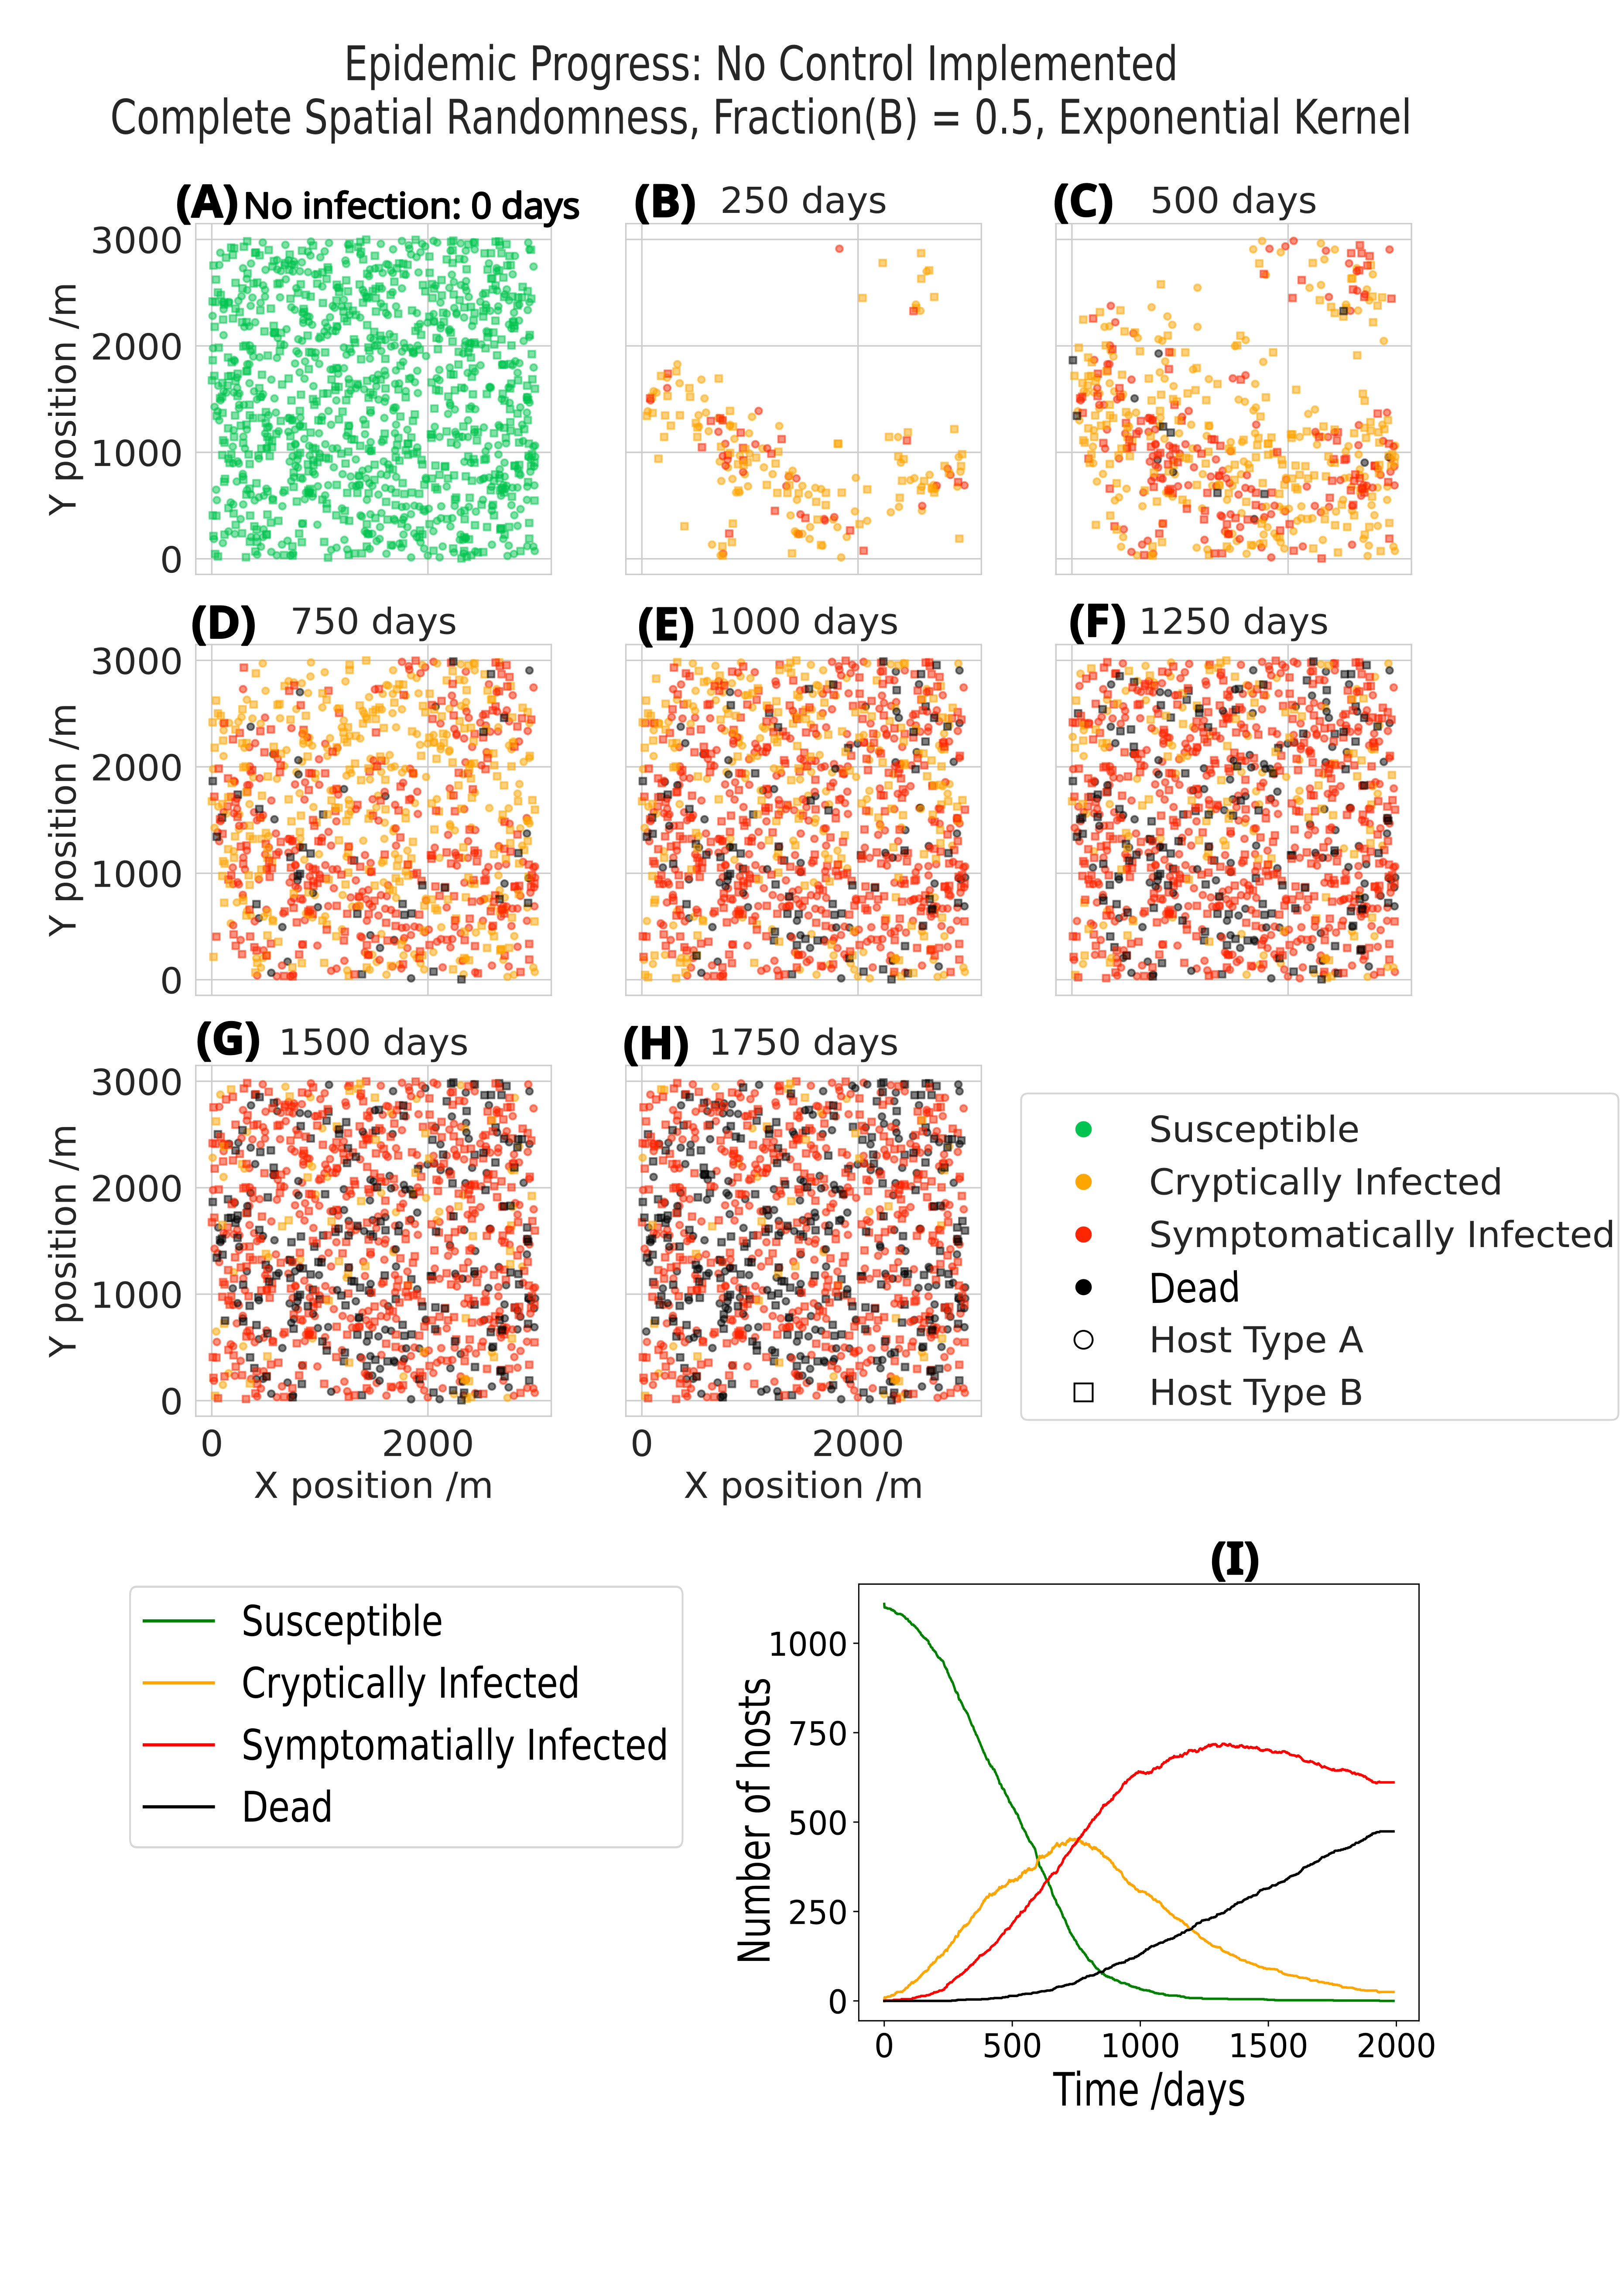
\includegraphics[width=0.854\textwidth]{dpc_highres.png}
	\caption{ \label{epi_nocontrol} \textbf{Progression of an epidemic in absence of disease control.} \textbf{(A)}: Susceptible (green) landscape before disease incursion begins. \textbf{(B)} $\rightarrow$ \textbf{(H)}: Following disease incursion, only Cryptic (orange), Symptomatic (red) and Dead (= Removed , black) hosts are shown for clarity.
		Half of hosts are type B (frac(B) = $\frac{1}{2}$) and approximately half the total hosts are infected by 500d (as expected under the normalisation condition). The epidemic front spreads in a wavelike manner across the landscape, infecting nearly all hosts by 1000 days. \textbf{(I)}: The disease progress curve corresponding to the epidemic shown in panels (B) to (H): Host deaths begin to be significant towards $T = 750$ days. Susceptible hosts are exhausted fully by $\approx$ 1500 days. The parameterisation is $\emph{Xylella}$-like. Host density $\approx 123$ hosts/km$^{2}$ (Medium Density Regime), and $N = 1110$.}
\end{figure}

\subsection*{Epidemic Metrics and Theoretical Foundations} 
Export of infectious material to areas outside the modelled square domain is a significant risk, and if the surrounding area has economic or cultural value, then successful control of invasive disease depends on reducing export of infectious material to the surrounding area. Area Under Disease Progress Curve (AUDPC) gives some measure of pathogen export \cite{Cunniffe2015} for an epidemic ending at time $\tau_{e}$: 
\begin{equation}
	\mathrm{AUDPC} = \int_{t = 0}^{\tau_{e}}\left( C(t) + I(t)\right)  dt  
\end{equation}
However, in a multi-type epidemic the infectivity of each host type, $\nu_{i}$, may differ. Hence, calculation of the modified AUDPC 
\begin{equation}
	\mathrm{AUDPC} = \int_{t = 0}^{\tau_{e}} \left( \sum_{i} \nu_{i} (I_{i}(t) + C_{i}(t)) \right) dt
\end{equation}
is used below.

I also remark that, modifying \cite{vandenBosch2024} slightly gives:

\begin{equation}
	R_{0, i} = \nu_{i} \Bigl(\frac{1}{\sigma_{i}} +  \frac{1} {\gamma} \Bigr)   \int_{0}^{\infty} \Bigl(  2 \pi r D(r) \left( O_i(r)\phi_{i} + O_{j}(r)\phi_{j} \right) \Bigr) dr
\end{equation}
for the basic reproductive number of a type $i$ host. The pathogen has dispersal kernel $D(r)$ and susceptible host type $i$ occurring with expected density $O_{i}(r)$ at distance $r$ from the infected host.  Then for a radius of control $\mathrm{r}_{\mathrm{removal}}$:

\begin{equation}
	\label{gnocont}
	R_{\mathrm{escaped}, 0} = \nu_{i} \Bigl(\frac{1}{\sigma_{i}} +  \frac{1} {\gamma} \Bigr) \int_{\mathrm{r}_\mathrm{removal}}^{L}  \Biggl( 2 \pi r D(r)\Bigl( O_i(r)\phi_{i} + O_{j}(r)\phi_{j} \Bigr)\Biggr) dr
\end{equation}

where $R_{\mathrm{escaped},0}$ gives the number of secondary infections established outside the host removal zone if the primary infected host were to be detected immediately. 

Eq. (\ref{gnocont}) provides an explanatory framework for the dynamics of epidemics at early time, but does not incorporate periodic surveying and radial removal processes.  Nevertheless, it provides testable predictions for the effect of landscapes on the epidemic. In particular, Eq. (\ref{gnocont}) predicts that the epidemic growth rate at early times is elevated for higher infectivity ($\nu$), and that control should be more challenging for thicker-tailed kernels. $R_0$ was not directly computed in the Monte Carlo simulations, as the basic reproductive number is of lesser importance compared to the $K_E$ and AUDPC. Furthermore, the best way to define $R_0$ in a radial host removal regime is unclear, as new infections may be rapidly removed. More relevant, then, is the survival time of hosts following infection and their infectivity as integrated by the type-corrected AUDPC.

\FloatBarrier
\section*{Results}

\subsection*{Q1, Q2: How does increasing proportion of cryptic host type B influence control?}

In general, an increase in both epidemic impact ($K_E$) and area under the disease progress curve (AUDPC) was observed as the fraction of cryptic host (type B) was increased. This trend persisted even if the control was optimised to the landscape considered. Two potential forms of crypticity were considered in turn: the first being when host types developed symptoms at the same rate ($\sigma_A = \sigma_B$) but symptoms on host type B are only detected with probability 0.2 ($p_{d,B} = 0.2$) and $p_{d,A}$ = 1. This can be abbreviated as the '$\Delta p_d$ case' and is examined before the alternative case of $\sigma_A > \sigma_B$ ('the $\Delta \sigma$ case'.)

To introduce the results of the two-dimensional parameter sweeps, it is helpful to consider the effect of varying control radius on a homogeneous landscape epidemics first. \textbf{Fig \ref{1d}} shows a 1-dimensional parameter sweep with a clear optimal radius of removal with respect to (w.r.t.) epidemic impact $K_E$ at approximately 400m. For this control radius, the median numnber of hosts spared infection or removal ($= N - K_E$) is maximised. At a low radius of removal ($r_\mathrm{rem}$ < 300m), the majority of hosts are infected. However, if  the radius of removal is too large (say $r_\mathrm{rem}$ > 450m), then an increase in $K_E$ is observed since excessive removal of uninfected hosts occurs. Because presence of a more cryptic host type in the landscape often changes the optimal radius of control, this one-drimensional parameter sweep was repeated with cryptic hosts present at increasing proportion to give the 2-dimensional scan (\textbf{Fig \ref{complex1}}). 

\begin{figure}[h]
	\centering
	\includesvg[width=\textwidth]{16km_response_smallerpts} % scaling to textwidth
	\vspace{10mm}
	\caption { \label{1d} \textbf{Median epidemic impact $K_E$ shows a clear optimum under varying radius of control but Area Under Disease Progress Curve (AUDPC) does not.} \textbf{(A)}: There is a relatively well-defined optimal radius of removal at approximately 400m with respect to epidemic impact $K_E$.   \textbf{(B)}: AUDPC is increased several-fold for a radius of removal < 250m compared to large (> 400m) radii of removal. For > 400m removal radius AUDPC displays a comparatively flat response value of 2 x 10$^{3}$, indicating no cost to increasing the removal radius with respect to AUDPC. Crucially, there is no obvious mapping between the $K_E$ and AUDPC outcome variables. Host density of 69.3 hosts /km$^{2}$ on a square landscape of type A hosts only, with 1110 total hosts. Blue shading indicates the percentile of stochastic replicates in which the y-value was attained, and brown dots show the median percentile. Parameterisation is for \emph{Xylella} with $\sigma_{A}$ = $\frac{1}{350}$ days$^{-1}$, with an exponential dispersal kernel. 1250 epidemics performed per point at 50 m step-size, with 250 replicates for each of 5 landscapes.}
	\vspace{10mm}
\end{figure}

\begin{figure}% this is the first complex figure
	\centering
	\includesvg[width=0.8\textwidth]{figure1_complex}
			\vspace{5mm}
	\caption{ \label{complex1} 
			\textbf{The effect of increasing the proportion of host type B, with $p_{d,B}  = 0.2$}. $\sigma_{A} = \sigma_{B} = \frac{1}{350}  \mathrm{days}^{-1}$. Epidemic metrics were computed for host landscapes of complete spatial randomness with $\approx 70 \: \mathrm{ hosts} / \mathrm{km}^2$. \textbf{(A)} The optimal radius of host removal generally increases as the proportion of cryptic hosts rises, when measuring the Median epidemic impact $K_E$. \textbf{(B)} The same epidemics as for A), but AUDPC computed as the dependent variable. Near-Optimal AUDPC is attainable for a far broader range of control radii than optimal $K_E$ is. Optimal radii show a less pronounced trend with a smaller impact on Median AUDPC. Each block is 250 replicates at a resolution of 50 m in panels (A) and (B). Panels \textbf{(C)} \& \textbf{(D)}: Both landscape-optimised and misspecified controls degrade in effectiveness(with respect to $K_{E}$ in \textbf{(C)} and AUDPC in \textbf{(D)})  as the proportion of cryptic ($p_{d,B} = 0.2$) hosts rises. \textbf{(C)} shows the close similarity in control efficacy between control strategies, as measured by $K_E$, as the fraction of host type B increases. \textbf{(D)}: The increase in AUDPC as (frac(B) $\rightarrow$ 1) is more pronounced for the misspecified control case, and exhibits significant divergence from landscape-adapted control as shown by the lack of overlap in interquartile ranges for frac(B) $>$ 0.5. }
\end{figure}

The epidemic impact $K_E$ showed a clear optimum (\textbf{Fig \ref{complex1}A}) at $r_{\mathrm{removal}} \approx$ 400m when only type A (olive-like) hosts were present. Under this control radius, approximately 550 hosts of 1110 were lost to removal or disease ($K_E = 550$). As the fraction of host type B increased, the optimal radius exhibited a nonlinear increase to a maximum of $\approx 750$ m, although for the landscapes composed mostly of host type B (i.e., frac(B) = 0.8 or 1.0) a significant majority of hosts ($K_E > 800$) were lost. Hence, increasing proportion of host type B damaged the radial control programme even under landscape-specific control radius optimisation to minimise $K_E$.  The AUDPC (\textbf{Fig \ref{complex1}B}) showed a weaker trend with a possible small increase in optimal radius from ~ 950m at frac(B) = 0 to $\approx$ 1150m at frac(B) = 1. The distributions of $K_E$ were more sharply-peaked than those of the AUDPC as response variable. This reflects the constraining cost associated with increasing removal radius, since more uninfected hosts are removed. By contrast, in the AUDPC case, a more aggressive control strategy with larger radius is rewarded, as there is no penalisation of excess host removals, and instead absolute minimisation of the infection pressure applied by the modelled patch is desired. The AUDPC was increased approximately 5-fold from maximal removal radius (1200m) and frac(B) = 0 (best-performing control) to frac(B) = 1 and $r_\mathrm{removal} = 0$m (worst-performing control). This equates approximately to a 5-fold range in pathogen export to the surroundings across all landscapes and control regime combinations considered. The 2D parameter scan approach also reveals the outcome if control radii are held constant to the minimal values for an all-A landscape and allows comparison with a control programme tailored to the specific mixture of A and B hosts present on the landscape. 


These two control strategies are termed the 'Misspecified' and 'Optimal' controls respectively, in \textbf{Fig \ref{complex1} (C), (D)} (and analogous later figures). \textbf{Fig. \ref{complex1}} panels \textbf{(C, D)} compare optimal control for each degree of host type heterogeneity with optimal control for frac(B) = 0. There is significant divergence between the optimal strategies when radius is optimised for $K_E$ compared to if radius were optimised for AUDPC. The misspecified control strategy (i.e., removal radius 400m) led to approximately twice the median AUDPC than for the lanscape optimised case when the landscape is all B hosts. However, the median $K_E$ exhibited closer correspondence between the landscape adapted case and the type A misspecified control case than median AUDPC response variable did. Specifically, in panel \textbf{(C)} the 25th, median and 75th percentiles of the $K_E$ exhibit close correspondence until frac(B) = 0.6, in contrast to the lack of overlap in AUDPC \textbf{(D)} for the same landscapes. In summary, for the $\Delta p_d$ case the increasing landscape fraction of more cryptic and misspecified hosts reduces the efficacy of control. 

\FloatBarrier

  \subsubsection*{Thicker-tailed kernels reduce efficacy of radial control and increase export risk under type-heterogeneous landscapes}
 
 The findings in \textbf{Fig. \ref{complex1}} were qualitatively robust to the form of the dispersal kernel. For the thick-tailed Cauchy kernel there was an increased $K_E$ relative to the exponential kernel, indicating that disease was harder to control, with an increased probability of dispersal events falling outside a given  control radius (see Eq. \ref{gnocont}). As the fraction of type B hosts increased, the optimal radius of removal with respect to $K_E$ also increased at a constant rate to a maximum at frac(B) = 1 (\textbf{Fig. {\ref{cauchycomplex}}}). Furthermore, comparison of landscape-optimised strategies with the naively misspecified control strategy (that is, optimal radius to minimise $K_E$ with frac(B) = 0), then no overlap in interquartile range between the two strategies was observed with respect to AUDPC (\textbf{Fig. \ref{cauchycomplex}D}). Importantly \textbf{Fig. \ref{cauchycomplex} C, D} shows that an adaptive radius of control on an increasingly type-heterogeneous landscape does not perform significantly better than the misspecified strategy, if $K_E$ is the response variable of interest. Hence, even knowing the exact fraction of each host on the landscape and optimising the removal radius to deal with this would not rescue a significant portion of healthy hosts. The qualitative findings with respect to $K_E$ are the same but this scenario is more challenging for disease control than \textbf{Fig. \ref{complex1}}. If AUDPC is measured, then the difference in performance between the optimal and misspecified strategies is significant (approximate twofold difference) even without presence of a second more cryptic host. The increase in frac(B) did little to change this difference, and so panel (\textbf{Fig. \ref{cauchycomplex}B}) represents a potential point of divergence from the previously examined exponential kernel case (\textbf{Fig. \ref{complex1}D}).
 
 \begin{figure}
 	\centering
 	\includesvg[width=0.8\textwidth]{cauchycomplex}
 		\caption{\label{cauchycomplex} \textbf{The Cauchy dispersal kernel reduces control efficacy but optimal radius of removal still increases with frac(B) $\rightarrow 1$.} \textbf{A)} Median epidemic impact ($K_{E}$) in the Cauchy kernel case is very high: approximately 900 of total 1110 hosts are infected or removed at optimum, even when all hosts are type A. Hence, control essentially fails in this case, for the given survey interval $\Delta = 90$ days. \textbf{(B)} shows that large radii of removal ($>1 $km) are favoured to reduce AUDPC to optimal values for nearly all landscapes considered. \textbf{(C)} and \textbf{(D)}: The thick-tailed Cauchy kernel exhibits marked divergence in AUDPC when misspecified control is used, compared to optimal control for the CSR landscape considered.  Note the upper-bounding of $K_E$ at high frac(B) since nearly all hosts are infected in either control radius strategy. \textbf{(B)} The AUDPC for control minimising $K_E$ is divergent from control minimising AUDPC, even without presence of two host types. A significant difference between the two distributions in AUDPC remains at increasing frac(B).}
 \end{figure}
 
  
 \FloatBarrier
 \subsection*{Q1, Q2: How does a longer cryptic period in host B affect control?}

  
The case where host B had a longer cryptic than A ($\Delta \sigma, \sigma_{B} < \sigma_{A}$) was also examined (\textbf{Fig \ref{sigma}}). The general increase in optimal radius of removal (w.r.t. epidemic impact $K_E$) as $\mathrm{frac(B)} \rightarrow 1$ was robust to whether the crypticity was a reduced probability of detection or a longer cryptic period.
However, with $\sigma_{B} = \frac{1}{500} \mathrm{days}^{-1}$ and $ p_{d,B} = 1$ there was a more modest and constant rate increase in the optimal radius with respect to $K_E$ (\textbf{Fig. \ref{sigma}A}) than for the previously treated $\Delta p_{d}$ case, which showed a nonlinear increase in optimal control radius (as frac(B) $\rightarrow 1$). At frac(B) = 1, here the optimal radius produced a median $K_E \approx 680$, but a large range of radii (350 - 700 m) gave similar $K_E$. This indicates a significant lack of system sensitivity to the radius of removal in that regime. Panel \textbf{(B)} shows that AUDPC also is quite unresponsive to the varying control radius, as long as it is above a threshold of $\approx 500$m. This corresponds with the $\Delta p_{d}$ case which also showed reduced AUDPC sensitivity to removal radius.

\textbf{Fig. \ref{sigma}C} shows an approximately linear increase in $K_E$ as frac(B) $\rightarrow 1$ for optimal and misspecified controls. There is extensive variance in the $K_E$ distributions as shown by the large interquartile ranges (IQRs). In addition, there is no clear constraint of the $K_E$ variance by susceptible host exhaustion, in contrast to what was noted for the Cauchy kernel case (\textbf{Fig. \ref{cauchycomplex}}). Both the optimal and misspecified control strategies produce similar outcomes as measured by $K_E$ (extensive overlap in IQR) (\textbf{Fig. \ref{sigma}C}). By contrast, \textbf{Fig. \ref{sigma}D} exhibits a clear divergence between control strategies although both median AUDPCS increase linearly. The difference increased as frac(B) $\rightarrow$ 1, and the AUDPC-optimal strategy was able to retain a comparatively low, constant AUDPC. Furthermore, the variance exhibited in distribution of AUDPC is smaller in the optimised control regime compared to the misspecified radius case, indicating tighter system control (reducing risk of a very severe outbreak).

\begin{figure}
	\centering
	\includesvg[width=0.8\textwidth]{figure2_complex}
	\caption{\label{sigma} \textbf{Optimal radii tend to increase with the fraction of host B  when $\sigma_B < \sigma_A$ and \textbf{$p_{d,A} = p_{d,B}$} = 1}. \textbf{(A):} Optimal radius with respect to $K_E$  shows a less pronounced increase as frac(B) $\rightarrow$ 1 than for the $\Delta p_{d}$  case (Fig. \ref{complex1}), increasing slightly from 350m to 500m as frac(B) $\rightarrow$ 1. \textbf{(B):} Optimal radius of removal with respect to AUDPC shows no clear trend and a flat response for most larger radii ($r_{\mathrm{rem}} > 500m$).
	 \textbf{(C):} Close correspondence between the misspecified and optimal control strategies persists even as $\mathrm{Frac(B)} \rightarrow 1$ when measuring $K_{E}$.  \textbf{(D)} With AUDPC as the response variable, there is significant divergence between the two strategies, even for the mostly homogeneous landscapes, with $\mathrm{Frac(B)}$ small. This is exacerbated for increasing frac(B), leading to a $>1.5$-fold increased AUDPC for the misspecified case.}
\end{figure}

\newpage
\FloatBarrier

\FloatBarrier
\subsection*{Q3: Asymmetric transmission can reduce control efficacy}

Since the susceptibility of host types may differ, parameter scans under asymmetric transmission were conducted. Specifically, the worse-case scenario from a disease control perspective was examined, where the more cryptic host type B was either more susceptible to infection.

The transmission matrix had form

\begin{equation}
	\begin{pmatrix}
		\nu_{A} & \phi_{A} \\
		\nu_{B} & \phi_{B}  \\
	\end{pmatrix} 
\newline
= \frac{1}{100}
	\begin{pmatrix}
	2 & 0.9 \\
	2 & 1.4 \\
\end{pmatrix} 
\end{equation}

such that 


\begin{equation}
	\begin{pmatrix}
		\nu_{A} \phi_{A}  & \nu_{A} \phi_{B}  \\
		\nu_{B} \phi_{A} & \nu_{B} \phi_{B} \\
	\end{pmatrix} \\
 = \frac{1}{100^2} \begin{pmatrix}
 1.8  & 2.8 \\
 1.8 & 2.8 \\
 \end{pmatrix} 
\end{equation}
 Hence, the rate of symptom emergence was the same for each type but the host type B was both less detectable when symptomatic and more susceptible to being infected. The infectivity of each type was the same and was set to 0.02 to fulfil the normalisation condition. In parameter terms: $p_{d,A} = 1, p_{d,B} = 0.2$; $\sigma_{A} = \sigma_{B} =\frac{1}{350}$ $\mathrm{days^{-1}}$


The increasing fraction of host type B modulated the expected epidemic impact and AUDPC in a significant way (\textbf{Fig. \ref{asymm}A, B}), causing a sharp increase in optimal radius and also exacerbating divergence between AUDPC in the misspecified and optimal control cases even at relatively low frac(B) (\textbf{Fig. \ref{asymm}}). This is significantly more pronounced than the \textbf{Fig. \ref{complex1}} case where both host types having the same (lower) susceptibility.  The range of AUDPC values attained is large ($\approx$ factor of 7) and is likely partially a result of the normalisation being performed for an all-A landscape, where the average susceptibility is low. The epidemic impact $K_E$ (\textbf{Fig. \ref{asymm}C}) shows dramatic increase from $\approx 500$ hosts at an all-A landscape, to infection or removal of the whole modelled population in the misspecified control case. The gradual reduction in interquartile ranges as frac(B) $\rightarrow$ 1 reflects this. The optimal control case does not fare much better, but manages to retain $\approx$ 200 healthy hosts at eradication. Considering AUDPC (\textbf{Fig. \ref{asymm}D}), the divergence between the optimal and misspecified controls is significant and attributable to increasing prevalence of the more susceptible type B host. This can be seen from the rapid loss of quartile overlap between the optimal and misspecified controls as frac(B) $\rightarrow$ 1. 
 \begin{figure}[h]
 	\centering
 	\includesvg[width=0.8\textwidth]{asym_complex}
 	\vspace{5mm}
 	\caption{\label{asymm} \textbf{Asymmetric transmission damages control efficacy when the more susceptible host type is more cryptic.} \textbf{(A):} The response of $K_E$ to increasing frac(B) with radius of control allowed to vary. The optimal radius of removal (hollow green square) shows a significant increase from 400 m to $\approx$ 750m as frac(B) $\rightarrow 1$. Approximately 550 hosts are lost to the epidemic when there are only A hosts but when the landscape consists only of type B hosts, approximately 800 hosts are lost. \textbf{(B):} There is extensive difference between the lowest and highest AUDPCs, and nearly all of the optimal radii wrt AUDPC are close to the maxmimum examined. \textbf{(C):} The median $K_E$ increases significantly from 500 hosts to either $\approx$  1100 hosts or 900 hosts depending on whether control is adapted to the landscape or not. \textbf{(D):} The optimised control retains a far lower AUDPC than the misspecified control for the majority of heterogeneous landscapes examined, and the two strategies correspond closely for the homogeneous landscape, frac(B) = 0. Interestingly the AUDPC shows a maximum at intermediate frac(B).}
\end{figure}
  
\section*{Discussion}

 I considered, using a small-scale modelling approach, the effect of knowledge and uncertainty coupled with host type heterogeneity on the efficacy of control. I showed that the presence of a second more cryptic host type having either lower symptom detectability ($\Delta p_d$) or longer cryptic period ($\Delta \sigma$) caused increased $K_E$ and Area Under Disease Progress Curve (AUDPC) in general (\textbf{Q1}). If the disease controller knew the density of the host landscape but did not know the parameters of the B host type (instead assuming all hosts had less cryptic A-like parameters), then this misspecified control further increased epidemic impact $K_E$ and AUDPC (\textbf{Q2}). For increased susceptibility of the type B host to infection by the \emph{Xylella}-like bacterium, the optimal radius increased rapidly with increasing frac(B) and control showed degradation even for frac(B) = 0.2 (\textbf{Q3}). 
 
 Control of \emph{Xylella fastidiosa} is likely to be conservative since it is a high-consequence disease: immediate local eradication is desirable, to reduce the risk of the disease getting established in the area or surroundings. This is necessary despite the extensive cultural value of olive trees. This has been seen in Italy with demarcated zones several-fold larger than the landscapes considered here \cite{Bragard2019}. Hence, I argue that the AUDPC is the more relevant outcome variable for the \emph{X. fastidiosa} subsp. \emph{pauca} for small or medium scales and therein lies the relevance of this study, since much existing work is based around optimising $K_E$ with comparatively less consideration of AUDPC. This work builds upon \cite{Cunniffe2015} in generalising the AUDPC to include infectivity, and reveals significant effects of asymmetric transmission on the AUDPC. 

\subsection*{Types of Crypticity}

Two different forms of crypticity were considered. In the absence of control, the expected time to death following infection is $\frac{1}{\sigma_{i}} + \frac{1}{\gamma}$. Hence, a longer cryptic period implies a longer infectious period on average. This marks an important difference between the two forms of crypticity considered. Reduced symptomaticity ($\Delta p_d$ in the model framework considered) does not affect host survival in the absence of control. 
 Nonetheless, the host types are likely well-mixed (see, for example, \textbf{Fig. \ref{landscapeexample} (A)}). Thus, in the $\sigma_{A} > \sigma_{B}$ case the less cryptic host type (A) can act a sentinel-like host w.r.t. type B (as explored in \cite{Lovell-Read2023} parameterised to \emph{X. fastidiosa}). However, for the parameterisation which I adopted here in the $\Delta \sigma$ case, the difference in cryptic period parameter is small, whereas in \cite{Lovell-Read2023} the sentinel host considered had $\sigma_{i} = \frac{1}{49}$ days $^{-1}$. However, since the host type A is the valuable crop in this case and $\frac{\sigma_{A}}{\sigma_{B}} < 2$ there are no effective sentinel hosts in this system.
An important question for the results' relevance is the extent to which different types of crypticity occur in real-world pathosystems, and whether they could both be present. Imperfect symptom detection can occur via a variety of mechanisms. In the case of Olive Quick Decline Syndrome, the desiccation of the tree is obvious. However, in a secondary (non-olive) species, symptoms of \emph{X. fastidiosa} infection could be more subtle. \emph{X. fastidiosa} does cause leaf scorch in documented cases of infected oleander trees growing next to olive groves \cite{Saponari2013}, but if wild plants are not properly inspected or inspected by non-professionals then $p_d < 1$ is possible. I have already observed that the $\Delta \sigma$ case is seen in sentinel-like systems.

Although the value chosen for $p_{d,B} = 0.2$ could be argued to be unreasonably low, I justify this by remarking that the case of $p_d < 1$ approximates the case where only a fraction of hosts are surveyed, especially for large populations and $p_d \approx \frac{1}{2}$ since the number of detection events is binomially distributed. The consideration of crypticity has not been exhaustive. In particular, more biologically relevant parameterisations include the use of a function to describe time-dependent infectivity based on increasing bacterial load through time. More simply, a multiplicative factor can be used to reduce infectivity while cryptic. This has been done in \cite{Cendoya2024}, for instance. Alternatively, it could be possible to assign this infectivity in a type-dependent manner, and otherwise retain the crypticity-related parameters as the same between types.

\subsection*{Incomplete Parameter Knowledge: Implications of Results for Disease Control}

I have shown that control optimised to a landscape of a single host type can be very suboptimal if the actual landscape is different. Hence, incomplete landscape knowledge can be a challenge to disease control programmes, and could cause failure. A striking illustration of this is for the asymmetric transmission case \textbf{Fig. \ref{asymm}D}, where even at frac(B) = 0.4 the risk of disease export ($\approx$ AUDPC) is more than doubled. A pre-emptive removal of the more susceptible B host type (as is performed under more complex control schemes \cite{HyattTwynam2017}) would then be very beneficial for reducing the chance of the epidemic spreading to adjacent areas.

Interestingly, when the fraction of host type B in the landscape = 1 (frac(B) = 1) this corresponds to the case of parameter misspecification, as partly treated in \cite{HyattTwynam2017}, since all hosts are the same but possess different parameters to those on which the control radius is chosen. In \cite{HyattTwynam2017} the authors found that, for a single-type model parameterised to citrus canker ($\sigma = \frac{1}{107}$ days $^{-1}$ and $\alpha = 36.1$ m) all control strategies degraded with respect to $K_E$ when $\sigma$ was mischaracterised. A significant point which can be seen from \textbf{Figs. \ref{complex1}-\ref{asymm}} is that the distribution of AUDPC is not trivially obtainable from the $K_E$ distribution. Since \cite{HyattTwynam2017} focused on the effect of parameter misspecification with respect to epidemic impact $K_E$, my work shows in addition to this how AUDPC changes under misspecified parameters. Furthermore, there has been comparatively little consideration in the literature of type-dependent detection probability $p_{d,i}$. $p_{d,i} < 1$ might be more relevant in the context of untrained surveyers. For instance, work examining sensitivity of citizen scientist inspection in the context of Acute Oak Decline infection enables estimates of $p_d$ \cite{Combes2025} and feed-back into more tightly parameterised mechanistic studies than the present work. An estimate of $p_d$ = 0.5 was used by \cite{Mastin2020} in a study of risk-based sampling. It would be important to consider to what extent cryptic landscape heterogeneity can be compensated for by risk-based sampling in a multi-host context, since here I only considered a simple, comprehensive sampling scheme. 

\subsection*{Vector Dynamics: Seasonality and Extent of Polyphagy}

The vector population has not been explicitly modelled in this work. Current understanding of \emph{P. spumarius} behaviour indicates that the nymphs feeds on herbaceous cover prior to moving to the crop canopy in late summer \cite{GimenezRomero2023}. In California, seasonal fluctations in infections from vectors to hosts are statistically significant \cite{Bodino2021b}. Under this behaviour, the dispersal kernel is likely to change through time. Seasonal fluctations occur on a shorter timescale than host death when there is no control (see \textbf{Fig. \ref{epi_nocontrol}I}). I have shown that at high radii of removal the AUDPC is minimised. This tallies well with \cite{Cunniffe2015}, where larger removal radii were found to favour short epidemic times and low AUDPC. For an arbitrarily large removal radius, perhaps beyond those directly tested here (> 1200m), the rapid extinction of an epidemic might then quench the effect of vector population fluctuations. A fast-slow approximation could then be used to approximate the full model to increase computational tractability.

\subsection*{Limitations of Spatial Scale}

I have examined control at a small scale (1100 hosts and approximately 16 km$^2$), but clearly this is not the only relevant scale for \emph{Xylella} epidemiology. This is indicated by all results with respect to the AUDPC variable, especially \textbf{Figs. \ref{cauchycomplex}}, \textbf{\ref{asymm}} panels \textbf{(B)}, where optimal radii to reduce inoculum export are close to the maximum examined (1200m). Preliminary sensitivity analysis increasing the number of hosts to 2000, 3000, 4000 and 5000 hosts on correspondingly larger landscapes (with the same densities) did not show a change in the median per-host $K_E$ or per-host AUDPC under consderved radius of removal. Hence, results relating to crypticity and asymmetric transmission likely hold for homogeneous landscapes of intermediate size (side length 5 km). This scaling argument, however, cannot be extended indefinitely without seriously considering the effect of host clustering, which can significantly modify the optimal control strategy. This has been seen with citrus canker \cite{Parnell2010}. In the specific case of \emph{X. fastidiosa}, if one considers transmission between olive groves then it can be argued via a network theory approach and consideration of long-distance dispersal events that eradication of \emph{X. fastidiosa} in Apulia is not possible \cite{Strona2017, Strona2020}. However, even in this case there is still a need to survey at the olive grove scale and radial control could still play an important role in slowing spread. Hence, these results still have bearing for slowing inter-grove spread of disease in a multi-type landscape.

For the landscapes considered here, a more accurate way to compute the export risk would be to take into account edge effects, specifically that the hosts in the centre of the modelled patch may contribute significantly less to export of infectious material out of the patch than those at the edges. None of the literature has to my knowledge implemented such a correction, and it would further add scale-dependent effects. 


\section*{Supplemental Information}


\begin{figure}[h]
	\centering
	\includesvg[width=0.8\textwidth]{sym3}
	\vspace{5mm}
	\caption{ \label{sym3} \textbf{Symmetric Transmission on the Medium-Density landscape with different cryptic periods.} $\sigma_A = \frac{1}{350}, \sigma_B = \frac{1}{500}$ and $p_{d,A} = p_{d,B} = 1$
		\textbf{(A):} The optimal radius of removal increases with respect to $K_E$ as frac(B) increases\textbf{(B)} \textbf{(C)} \textbf{(D)} Host density $\approx$ 123 hosts /km$^2$. }
	\end{figure}



\begin{figure}[h]
	\centering
	\includesvg[width=0.8\textwidth]{asym3}
	\vspace{5mm}
	\caption{\label{asym3} \textbf{Asymmetric transmission on the Medium-Density Landscape, with different cryptic periods. } The type B host is parameterised as being higly susceptible to infection $\phi_{B}$ =  \textbf{(A)}  \textbf{(B)} \textbf{(C)} \textbf{(D)} Host density $\approx$ 123 hosts /km$^2$. }
\end{figure}

\subsection*{Code}

All relevant code, including the primary simulation tool, landscape generators and plotting scripts, are available at ... [TBD] \hyperbaseurl{https://github.com/vargasrichards/IIproj}



\section*{Acknowledgments}

I thank Prof. Nik Cunniffe for his careful and encouraging supervision, and members of the Cunniffe group for stimulating discussion. 

%
%\clearpage

\printbibliography
 

\end{document}